\section{Process}

In this section, we briefly review the architecture of the system for gathering and storing temperature sensor data, and then explain the setup of the parameter estimation problem using iterative proportional fitting.

\if 0
do we need this?
Approach: "quick" overview section
- explicitly what we're going to do
- how we're going to do it
- "now we go into more detail" etc

Architecture of System:
- sensors, database:
    - KETI and the Soda deployment
- data processing pipeline:
    - need for data cleaning; complications w/ sensors ('real world')
    - how to do data cleaning, the transformations we did
- Octave script to run IPF, generate edge parameters:
    - what would the results look like and what would we expect?

Problem Setup:
- how do decompose the space, the buildings, etc we used into graph
- go over options in how we could have represented:
    - bucketing temperature
    - more nodes; more accurate? more sensors
\fi



\subsection{Architecture}

\begin{figure}[ht]
\centering
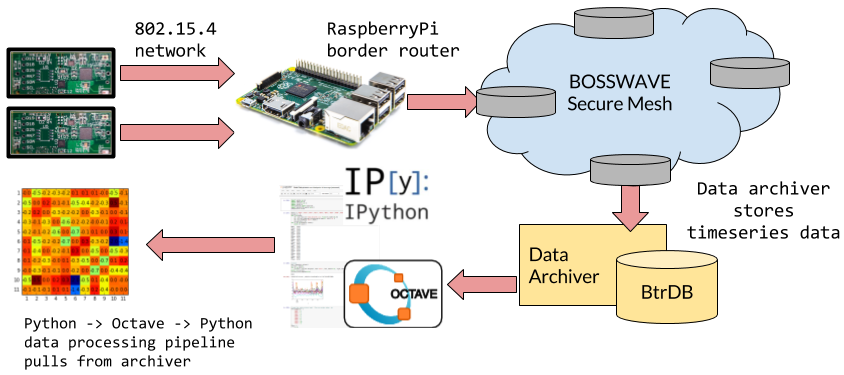
\includegraphics[width=.8\linewidth]{figs/281arch}
\caption{Overview of data acquisition and processing pipeline}
\label{fig:architecture}
\end{figure}

\begin{figure}[ht]
\centering
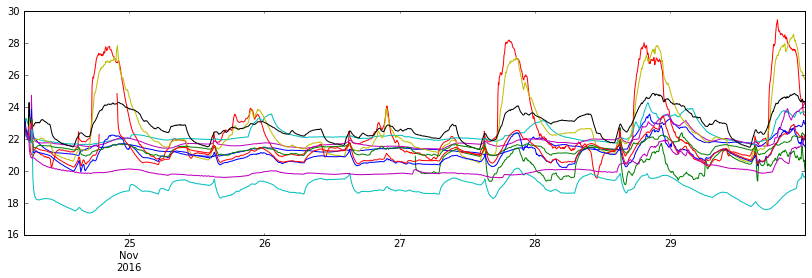
\includegraphics[width=.8\linewidth]{figs/temperatureplot}
\caption{Temperature of the 11 motes in the south-west corner of AMPlab during the week 11/24/2016 to 11/30/2016. The two weekend days are clearly visible, and a good amount of temperature correlation is visible across the traces.}
\label{fig:temperature}
\end{figure}

\textbf{Sensor Infrastructure:} For long-term distributed temperature sensing, we use the Hamilton sensor mote, recently developed at UC Berkeley by Michael Andersen~\cite{hamiltonmote}.
The Hamilton mote has a low-cost, low-power temperature sensor which it samples at a rate of .1 Hz (once every 10 seconds); the mote is duty-cycled at a rate projected to have it last on a single CR123 battery for over 3 years.
Each mote sends each temperature reading to a 802.15.4 border router running on a RaspberryPi 3, which forwards the message into a secure publish-subscribe network called BOSSWAVE~\cite{andersen2016enabling}.
From here, we have fine-grained control over which services and individuals can access the temperature data.

\textbf{Data Processing Pipeline:} The above process publishes sensor readings so that they may be consumed, but it does not actually save the data anywhere.
This is handled by the pundat~\cite{pundat} service which saves data in the BtrDB timeseries database~\cite{andersen2016btrdb}.
Using a set of client bindings, we can retrieve data for any set of sensors for any range of time.
This raw data was downloaded once, and then transformed by a set of Python and Octave scripts to do the data aggregation and iterative proportional fitting respectively.

For this paper, we retrieve all the raw temperature data for the 11 Hamilton motes in the south-west corner of the AMP lab for the week of 11/24/2016 to 11/30/2016; this is roughly 48,000 data points per sensor.
Figure~\ref{fig:temperature} contains a plot of the raw data.
This plot tells us two things: firstly, that there are many shared trends in the measured temperature (e.g. groups of motes tend to go up or down together).
Secondly, that the difference between two streams is likely an important differentiator, which we do not capture in our simple binary Ising model.
Exploring the \emph{value} of a temperature reading as an indicator for thermal coupling rather than just the sign of the gradient will be the focus of future work.

\subsection{Problem Setup}

We implement iterative proportional fitting (IPF, first introduced in \cite{deming1940least}) for the two pairwise Markov Random Fields representing the AMPlab microzones (Figure~\ref{fig:soda_edges}).
The factorizations of the MRFs are each given by:

\begin{equation}
P(x_1,\ldots,x_{11}) = \prod_{(i,j) \in E} \exp\lbrace W_{ij}x_ix_j\rbrace
\end{equation}

where $W_{ij}$ is the matrix from Equation~\ref{eq:W}.
Which graphical structure we use determines the edge set $E$, which will come from either the physical model or the fully-connected model.

To run IPF and estimate the edge parameters $W_{ij}$, we need to choose our dataset.
The raw temperature readings constantly fluctuate -- they are accurate to 0.1 Celsius -- and thus are too noisy to be considered in the binary Ising model.
We smooth the temperature data by applying an aggregation function (we explored \texttt{max}, \texttt{min} and \texttt{mean}) to various window sizes over the data: 30 seconds, 1 minute, 5 minute, 10 minute and 30 minute.
We predict that the higher the degree of aggregation, the more certain our found parameters will be, but we will lose any subtler interactions between nodes that would have been visible in finer-grained data.

Because of the large number of nodes and datapoints, we iterate our IPF implementation until successive iterations have a difference of less than $1 \times 10^{-8}$; this is enough to capture the sign and relative magnitudes of the found edge parameters.
